\documentclass[11pt]{article}
\usepackage{amsmath, amsthm, amsfonts,amssymb}
\usepackage[utf8]{inputenc}
\usepackage[spanish]{babel}
\usepackage{multicol}
\usepackage{listings}
\lstset{basicstyle=\footnotesize\ttfamily,breaklines=true}
\usepackage{alltt}
\usepackage{graphicx}
\usepackage{subfigure}
\usepackage{subfig}
\usepackage{float}
\usepackage{url}
\usepackage{enumerate}
\usepackage{framed}
\usepackage{color}
\usepackage{wrapfig}\definecolor{shadecolor}{RGB}{250,250,250}
\usepackage{framed}
\usepackage{epstopdf}
\setlength\parindent{0pt}
\usepackage{listings}
\usepackage{color} %red, green, blue, yellow, cyan, magenta, black, white
% Operadores matemáticos y simbolos
\DeclareMathOperator{\dive}{div}
\DeclareMathOperator{\trace}{trace}
\DeclareMathOperator{\tr}{tr}
\DeclareMathOperator{\symm}{symm}
\DeclareMathOperator{\sk}{skew}
\DeclareMathOperator{\grad}{grad}
\DeclareMathOperator{\Grad}{Grad}
\DeclareMathOperator{\curl}{curl}
\DeclareMathOperator{\Curl}{Curl}
\def\R{\mbox{\(\mathbb{R}\)}}
\def\E{\mbox{\(\mathbb{E}\)}}
\def\P{\mbox{\(\mathbb{P}\)}}
\def\I{\mbox{\(\mathbb{I}\)}}
\def\L{\mbox{\(\mathbb{L}\)}}
\def\dx{\mbox{\(\,\mathrm{d}x\)}}
\usepackage{geometry}
\geometry{left=2.5cm, right=2.5cm, top=2cm, bottom=3cm}
\begin{document}
\begin{figure}
\begin{minipage}{2.5cm}

\includegraphics[width=0.8\textwidth]{./figures/LogoUC-BN}
\end{minipage}
\begin{minipage}{14.5cm}
\vspace{4mm}
{\sc PONTIFICIA UNIVERSIDAD CAT\'OLICA DE CHILE}\\
{\sc Escuela de ingeniería} \\
ICS3153 \ Optimización Avanzada\\
Profesor: Cristóbal Guzmán (crguzmanp@uc.cl) \\
Alumno: Alberto Valdés (anvaldes@uc.cl) \\

\vspace{-8mm}
\hrulefill
\end{minipage}
\end{figure}
\phantom{""}
\vspace{-10mm}
\normalsize

\begin{center}
	\huge{Tarea 1}\\
	\normalsize 
\end{center}

\section*{Pregunta 1}

a) Como nos piden demostrar que (i), (ii) y (iii) son equivalentes, entonces los que haremos sera demostrar que: \\

(iii) $ \Rightarrow $ (ii)

(ii) $ \Rightarrow $ (i)

(i) $ \Rightarrow $ (iii) \\

Partiremos con: \\

\underline{(iii) $ \Rightarrow $ (ii):} \\

Sean $x,y \in \mathcal{X}$ arbitrarios, por (iii) tenemos que:

\[ \langle \nabla f(y) - \nabla f(x), y-x \rangle \geq \sigma \left\| y-x \right\|^{2} \]

$ \Rightarrow $ \

\[ \langle \nabla f(y), y-x \rangle - \langle  \nabla f(x), y-x \rangle  \geq \sigma \left\| y-x \right\|^{2} \]

$ \Rightarrow $ \

\[ \langle \nabla f(y), y-x \rangle   \geq \sigma \left\| y-x \right\|^{2} + \langle  \nabla f(x), y-x \rangle \ \ \ \ (1) \] \

Ahora definiremos $ g(t) = f(tx+[1-t]y) \ \Rightarrow \ g(0) = f(y), g(1) = f(x) $ \\

Notemos que $ g'(t) = \langle \nabla f(tx+[1-t]y),x-y \rangle $ \\

Ahora: 

\[ f(y) - f(x) = g(0) - g(1) = \int_{1}^{0} g'(t) dt = \int_{0}^1 - g'(t)dt = \int_{0}^1 - \langle \nabla f(tx+[1-t]y),x-y \rangle dt \]

\[ = \int_{0}^1 \langle \nabla f(tx+[1-t]y),y-x \rangle dt \]

$ \Rightarrow $ 

\[ f(y) - f(x) = \int_{0}^1 \langle \nabla f(tx+[1-t]y),y-x \rangle dt \ \ \ \ (2) \]

Usaremos $(1)$ reemplazando $y$ por $ tx + [1-t]y $ y manteniendo $x$. \\

De este modo:

\[ \langle \nabla f(tx + [1-t]y), (tx + [1-t]y)-x \rangle   \geq \sigma \left\| (tx + [1-t]y)-x \right\|^{2} + \langle  \nabla f(x), (tx + [1-t]y)-x \rangle \ \ \ \ (3) \]

Ahora notemos que:

\[ (tx + [1-t]y)-x = tx - x + [1-t]y = [t-1]x + [1-t]y = [1-t]y - [1-t]x = (1-t)(y-x) \]

De este modo $(3)$ nos queda como sigue: 

\[ \langle \nabla f(tx + [1-t]y), (1-t)(y-x) \rangle   \geq \sigma \left\| (1-t)(y-x) \right\|^{2} + \langle  \nabla f(x), (1-t)(y-x)\rangle  \]

$ \Rightarrow $ 

\[ (1-t) \langle \nabla f(tx + [1-t]y), y-x \rangle   \geq (1-t)^2 \sigma \left\| y-x \right\|^{2} + (1-t) \langle  \nabla f(x), y-x \rangle  \]

Consideremos $ t \neq 1 $, de esta forma:

\[  \langle \nabla f(tx + [1-t]y), y-x \rangle   \geq (1-t) \sigma \left\| y-x \right\|^{2} +  \langle  \nabla f(x), y-x \rangle \ \ \ \ (4) \]

Usando $(2)$ y $(4)$ llegamos a que:

\[ f(y) - f(x) = \int_{0}^1 \langle \nabla f(tx+[1-t]y),y-x \rangle dt \geq \int_{0}^{1} [(1-t) \sigma \left\| y-x \right\|^{2} +  \langle  \nabla f(x), y-x \rangle] dt \]

\[ = \sigma \left\| y-x \right\|^{2} \int_{0}^{1} (1-t) dt  +  \langle  \nabla f(x), y-x \rangle \int_{0}^{1} dt = \sigma \left\| y-x \right\|^{2} \left( t - \frac{t^2}{2} \big]_{0}^{1} \right)  +  \langle  \nabla f(x), y-x \rangle  \]

\[ = \sigma \left\| y-x \right\|^{2} \left( 1 - \frac{1}{2}  \right)  +  \langle  \nabla f(x), y-x \rangle = \sigma \left\| y-x \right\|^{2} \frac{1}{2}  +  \langle  \nabla f(x), y-x \rangle = \frac{\sigma}{2} \left\| y-x \right\|^{2}  +  \langle  \nabla f(x), y-x \rangle \]

$ \Rightarrow $ 

\[ f(y) - f(x) \geq \frac{\sigma}{2} \left\| y-x \right\|^{2}  +  \langle  \nabla f(x), y-x \rangle \]

$ \Rightarrow $ 

\[ f(y) \geq f(x) + \langle  \nabla f(x), y-x \rangle + \frac{\sigma}{2} \left\| y-x \right\|^{2}  \ \ \ (5)  \] \

Y como se tomaron $ x,y \in \mathcal{X} $ arbitrarios entonces:

\[ f(y) \geq f(x) + \langle  \nabla f(x), y-x \rangle + \frac{\sigma}{2} \left\| y-x \right\|^{2} \ \ \ \forall x,y \in \mathcal{X} \]

Y esta desigualdad es justamente a la que queríamos llegar, es decir (ii). \\

De este modo, se demostró que $ \boxed{(iii)  \Rightarrow  (ii)} $. \

\hrulefill

$ \ $ 

\underline{(ii) $ \Rightarrow $ (i):} \\

Consideremos $x,y \in \mathcal{X}$ arbitrarios, notemos que por $ (ii) $ tenemos que:

\[ f(y) \geq f(x) + \langle \nabla f(x), y-x \rangle + \frac{\sigma}{2} \left\| y-x \right\|^{2} \ \ \ \ (6) \]

Definimos $ x_{\lambda} = \lambda x + [1-\lambda] y $ con $ \lambda $: $ 0 \leq \lambda \leq 1 $ \\

Reemplazando $ x $ por $ x_{\lambda} $ y manteniendo $y$ tenemos que por $(6)$ se da la siguiente desigualdad:

\[ f(y) \geq f(x_{\lambda}) + \langle \nabla f(x_{\lambda}), y-x_{\lambda} \rangle + \frac{\sigma}{2} \left\| y-x_{\lambda} \right\|^{2}  \] \

Notemos que $ y - x_{\lambda} = y - \lambda x - (1-\lambda)y = y - \lambda x - y + \lambda y = \lambda(y-x) $ \\

De esta modo:

\[ f(y) \geq f(\lambda x + [1-\lambda] y) + \langle \nabla f(\lambda x + [1-\lambda] y), \lambda(y-x) \rangle + \frac{\sigma}{2} \left\| \lambda(y-x) \right\|^{2}  \]

$ \Rightarrow $ 

\[ f(y) \geq f(\lambda x + [1-\lambda] y) + \lambda \langle \nabla f(\lambda x + [1-\lambda] y), y-x \rangle + \lambda ^2 \frac{\sigma}{2} \left\| y-x \right\|^{2}  \ \ \ \ (7) \]

Reemplazando $ y $ por $ x $ y $ x $ por $ x_\lambda $ en $(6)$ obtenemos que:

\[ f(x) \geq f(x_\lambda) + \langle \nabla f(x_\lambda), x-x_\lambda \rangle + \frac{\sigma}{2} \left\| x-x_{\lambda} \right\|^{2} \ \ \ \ (8) \]

Notemos que:

\[ x - x_{\lambda} = x - [\lambda x + (1-\lambda) y] = x - \lambda x - (1-\lambda)y = (1-\lambda)x-(1-\lambda)y = (1-\lambda) (x-y) \]

Reemplazando en $(8)$ llegamos a que:

\[ f(x) \geq f(\lambda x + [1-\lambda] y) + \langle \nabla f(\lambda x + [1-\lambda] y), (1-\lambda)(x-y) \rangle + \frac{\sigma}{2} \left\| (1-\lambda) (x-y) \right\|^{2} \ \ \ \ (8) \]

$ \Rightarrow \ $ 

\[ f(x) \geq f(\lambda x + [1-\lambda] y) + (1-\lambda)\langle \nabla f(\lambda x + [1-\lambda] y), x-y \rangle + (1-\lambda)^2 \frac{\sigma}{2} \left\|  x-y \right\|^{2} \ \ \ \ (9) \] \

\newpage

Ahora multiplicando $(7)$ por $(1-\lambda)$ y sumándola a $ \lambda $ por $(9)$ obtenemos que:
 
\[ (1-\lambda)f(y) + \lambda f(x) \geq (1-\lambda) f(\lambda x + [1-\lambda] y) + \lambda f(\lambda x + [1-\lambda] y) + (1-\lambda) \lambda \langle \nabla f(\lambda x + [1-\lambda] y), y-x \rangle \]

\[ + \lambda (1-\lambda)\langle \nabla f(\lambda x + [1-\lambda] y), x-y \rangle + (1-\lambda) \lambda ^2 \frac{\sigma}{2} \left\| y-x \right\|^{2} + \lambda (1-\lambda)^2 \frac{\sigma}{2} \left\|  x-y \right\|^{2} = \]

\[  f(\lambda x + [1-\lambda] y) + (1-\lambda) \lambda \langle \nabla f(\lambda x + [1-\lambda] y), y-x \rangle - \lambda (1-\lambda)\langle \nabla f(\lambda x + [1-\lambda] y), y-y \rangle + (1-\lambda)\lambda [\lambda + (1-\lambda)] \frac{\sigma}{2} \left\| y-x \right\|^{2} \]

\[ = f(\lambda x + [1-\lambda] y) +   \frac{\sigma (1-\lambda)\lambda }{2} \left\| y-x \right\|^{2} \] 

$ \Rightarrow $ 

\[ (1-\lambda)f(y) + \lambda f(x) \geq f(\lambda x + [1-\lambda] y) +   \frac{\sigma (1-\lambda)\lambda }{2} \left\| y-x \right\|^{2} \]

$ \Rightarrow $ 

\[ (1-\lambda)f(y) + \lambda f(x) - \frac{\sigma (1-\lambda)\lambda }{2} \left\| y-x \right\|^{2} \geq f(\lambda x + [1-\lambda] y)    \]

$ \Rightarrow $ 

\[ f(\lambda x + [1-\lambda] y) \leq \lambda f(x) + (1-\lambda)f(y) - \frac{\sigma (1-\lambda)\lambda }{2} \left\| y-x \right\|^{2}  \] \

Y como se tomo $ x,y \in \mathcal{X} $ arbitrarios, además de que el $ \lambda $ es tal que $ 0 \leq \lambda \leq 1 $, entonces:

\[ f(\lambda x + [1-\lambda] y) \leq \lambda f(x) + (1-\lambda)f(y) - \frac{\sigma (1-\lambda)\lambda }{2} \left\| y-x \right\|^{2} \ \ \ \forall x,y \in \mathcal{X}, \forall \lambda: 0 \leq \lambda \leq 1  \]

Y esta desigualdad es justamente a la que queríamos llegar, es decir (i). \\

De este modo, se demostró que $ \boxed{(ii)  \Rightarrow  (i)} $. \

\hrulefill

$ \ $ 

\underline{$(i) \Rightarrow (iii) $}: \\

Sean $ x,y \in \mathcal{X} $ arbitrarios y $ \lambda $ arbitrario tal que $ 0 \leq \lambda \leq 1 $, por (i) tenemos que: 

\[ f(\lambda x + [1-\lambda] y ) \leq \lambda f(x) + [1-\lambda] f(y) - \frac{\sigma \lambda (1-\lambda)}{2} \left\| y-x \right\|^{2}  \]

$ \Rightarrow $ 

\[ f(\lambda x + [1-\lambda] y ) \leq \lambda f(x) + f(y) - \lambda f(y) - \frac{\sigma \lambda (1-\lambda)}{2} \left\| y-x \right\|^{2}  \]

$ \Rightarrow $ 

\[ f(\lambda x + [1-\lambda] y ) - f(y) \leq \lambda f(x)  - \lambda f(y) - \frac{\sigma \lambda (1-\lambda)}{2} \left\| y-x \right\|^{2}  \]

Consideremos un $ \lambda \neq 0 $ y como $ 0 \leq \lambda \leq 1 $, entonces estamos considerando un $ \lambda > 0 $ \\

$ \Rightarrow $ 

\[ \cfrac{f(\lambda x + [1-\lambda] y ) - f(y)}{\lambda} \leq  f(x)  -  f(y) - \frac{\sigma  (1-\lambda)}{2} \left\| y-x \right\|^{2}  \]

Como estamos considerando un $ \lambda > 0 $ entonces sacaremos el limite de cuando $ \lambda $ tiene a $0$ por la derecha. De este modo:

\[  \lim_{\lambda \to 0^+} \left[ \cfrac{f(\lambda x + [1-\lambda] y ) - f(y)}{\lambda} \right] \leq \lim_{\lambda \to 0^+} \left[ f(x)  -  f(y) - \frac{\sigma  (1-\lambda)}{2} \left\| y-x \right\|^{2}  \right] \ \ \ \ (10) \] \

$ \ $ 

Ahora como $ f $ es diferenciable sobre $ \mathcal{X}$, entonces: \\

\[ \lim_{\lambda \to 0^+} \left[ \cfrac{f(\lambda x + [1-\lambda] y ) - f(y)}{\lambda} \right] = \lim_{\lambda \to 0} \left[ \cfrac{f(\lambda x + [1-\lambda] y ) - f(y)}{\lambda} \right] =  \]

\[ \lim_{\lambda \to 0} \left[ \cfrac{f(y + \lambda (x-y) ) - f(y)}{\lambda} \right] = \langle \nabla f(y), x-y \rangle \] \\

Y reemplazando esto en $(10)$ llegamos a que:

\[   \langle \nabla f(y), x-y \rangle \leq \lim_{\lambda \to 0^+} \left[ f(x)  -  f(y) - \frac{\sigma  (1-\lambda)}{2} \left\| y-x \right\|^{2}  \right] \ \ \ \ (11) \] \

Ahora notemos que:

\[ \lim_{\lambda \to 0^+} \left[ f(x)  -  f(y) - \frac{\sigma  (1-\lambda)}{2} \left\| y-x \right\|^{2}  \right]  = f(x)  -  f(y) - \frac{\sigma}{2} \left\| y-x \right\|^{2}  \] \\

Y reemplazando esto en $(11)$ llegamos a que: \

\[   \langle \nabla f(y), x-y \rangle \leq f(x)  -  f(y) - \frac{\sigma}{2} \left\| y-x \right\|^{2} \ \ \ \ (12) \] \

Como se tomo $x,y \in \mathcal{X} $ arbitrarios entonces:

\[   \boxed{\langle \nabla f(y), x-y \rangle \leq f(x)  -  f(y) - \frac{\sigma}{2} \left\| y-x \right\|^{2} \ \ \ \forall x,y \in \mathcal{X} \ \ \ (13)} \] \

Ahora como el $x$ y el $y$ son arbitrarios entonces la desigualdad anterior también es valida si reemplazamos $ x $ por $ y $, además de reemplazar $ y $ por $x$ \

\[   \langle \nabla f(x), y-x \rangle \leq f(y)  -  f(x) - \frac{\sigma}{2} \left\| x-y \right\|^{2}   \ \ \ \ (14) \] \

\newpage

Ahora si sumamos $(12)$ y $(14)$ llegamos a que:

\[ \langle \nabla f(x), y-x \rangle + \langle \nabla f(y), x-y \rangle \leq f(x)  -  f(y) - \frac{\sigma}{2} \left\| y-x \right\|^{2} +  f(y)  -  f(x) - \frac{\sigma}{2} \left\| x-y \right\|^{2} \ \ \ \ (15) \]

Notemos que:

\[ \langle \nabla f(x), y-x \rangle + \langle \nabla f(y), x-y \rangle = \langle \nabla f(x), y-x \rangle - \langle  \nabla f(y), y-x \rangle \]

\[ = \langle \nabla f(x) - \nabla f(y), y-x \rangle = - \langle \nabla f(y) - \nabla f(x), y-x \rangle \] \

Reeemplazando esto en $(15)$ llegamos a que:

\[ - \langle \nabla f(y) - \nabla f(x), y-x \rangle \leq f(x)  -  f(y) - \frac{\sigma}{2} \left\| y-x \right\|^{2} +  f(y)  -  f(x) - \frac{\sigma}{2} \left\| x-y \right\|^{2} \ \ \ \ (16) \] \

Además tenemos que:

\[  f(x)  -  f(y) - \frac{\sigma}{2} \left\| y-x \right\|^{2} +  f(y)  -  f(x) - \frac{\sigma}{2} \left\| x-y \right\|^{2} = - \frac{\sigma}{2} \left\| y-x \right\|^{2} - \frac{\sigma}{2} \left\| x-y \right\|^{2}  \]

\[ = - \frac{\sigma}{2} \left\| y-x \right\|^{2} - \frac{\sigma}{2} \left\| y-x \right\|^{2} = - \sigma \left\| y-x \right\|^{2}  \] \

Reemplazando esto en $(16)$ llegamos a que:

\[ - \langle \nabla f(y) - \nabla f(x), y-x \rangle \leq - \sigma \left\| y-x \right\|^{2} \] 

$ \Rightarrow $ 

\[  \langle \nabla f(y) - \nabla f(x), y-x \rangle \geq  \sigma \left\| y-x \right\|^{2} \] \

Como desde un inicio habíamos tomado $x,y \in \mathcal{X}$ arbitrarios, entonces:

\[  \langle \nabla f(y) - \nabla f(x), y-x \rangle \geq  \sigma \left\| y-x \right\|^{2} \ \ \forall x,y \in \mathcal{X} \]  \

Y esta desigualdad es justamente a la que queríamos llegar, es decir (iii). \\

De este modo, se demostró que $ \boxed{(i)  \Rightarrow  (iii)} $. \\

Así finalmente como se demostró que: \\

$ (iii)  \Rightarrow  (ii) $ \\
$ (ii)  \Rightarrow  (i) $ \\
$ (i)  \Rightarrow  (iii) $ \\

Entonces se demostró que $(i),(ii)$ y $(iii)$ son equivalentes. \\
 
\hrulefill

$ \ $ \

b) Nos piden demostrar que sea $ f: \mathcal{X} \rightarrow \mathbb{R} $ de clase $ \mathcal{C}^{2} $ sobre $ \mathcal{X}$, entonces es $ \sigma$-fuertemente convexa si y solo si: 

\[ \langle h, \nabla^2 f(x) h \rangle \geq \sigma \left\| h \right\|^{2} \ \ \ \forall x \in Dom(f), \forall h \in \mathbb{R}^d \] \

Como nos piden demostrar un $ \Leftrightarrow $ entonces demostraremos primero $ \Rightarrow $ y luego $ \Leftarrow $ \\

\textbf{Nota:} Ahora comenzaremos a enumerar nuevamente a las ecuaciones desde el $(1)$ hacia arriba y no se consideraran las ecuaciones de la parte $a)$. \\

\underline{$ \Rightarrow $}: \\

Como $f$ es $\sigma$-fuertemente convexa, entonces:

\[ \langle \nabla f(y) - \nabla f(x),y-x \rangle \geq \sigma \left\| y-x \right\|^{2}  \]

$ \Rightarrow $ 

\[ \langle \nabla f(y) ,y-x \rangle - \langle \nabla f(x) ,y-x \rangle  \geq \sigma \left\| y-x \right\|^{2} \ \ \ (1) \] \

Tomamos $ y = x + th \ \Rightarrow \ y - x = th \ \Rightarrow \ \left\| y-x \right\|^{2} = \left\| th \right\|^{2} = t^2 \left\| h \right\|^{2} $ \\

Reemplazando en $(1)$ nos queda que: \

\[ \langle \nabla f(x+th) ,th \rangle - \langle \nabla f(x) ,th \rangle  \geq \sigma t^2\left\| h \right\|^{2} \]

$ \Rightarrow $ 

\[ t [\langle \nabla f(x+th) ,h \rangle - \langle \nabla f(x) ,h \rangle]  \geq \sigma t^2\left\| h \right\|^{2} \] \

Consideremos $ t \neq 0 $, entonces tenemos que:

\[  [\langle \nabla f(x+th) ,h \rangle - \langle \nabla f(x) ,h \rangle]  \geq \sigma t \left\| h \right\|^{2} \] \

Ahora consideremos a $ t > 0 $, de este modo: \\

\[  \cfrac{\langle \nabla f(x+th) ,h \rangle - \langle \nabla f(x) ,h \rangle}{t}  \geq \sigma \left\| h \right\|^{2} \]

\newpage

Ahora, como se considero $ t > 0 $ entonces podemos aplicar a ambos lados el limite cuando $ t $ tiende a $ 0 $ por la derecha, de este modo: \\

\[  \underset {t \to 0^+} {l \acute{\imath}m} \left[ \cfrac{\langle \nabla f(x+th) ,h \rangle - \langle \nabla f(x) ,h \rangle}{t}  \right] \geq   \underset {t \to 0^+} {l \acute{\imath}m} \left[ \sigma \left\| h \right\|^{2} \right] \ \ \  (2) \] \

Es claro que:

\[ \underset {t \to 0^+} {l \acute{\imath}m} \left[ \sigma \left\| h \right\|^{2} \right] = \sigma \left\| h \right\|^{2} \] \ 

Reemplazando en $(2)$ nos queda que: \


\[  \underset {t \to 0^+} {l \acute{\imath}m} \left[ \cfrac{\langle \nabla f(x+th) ,h \rangle - \langle \nabla f(x) ,h \rangle}{t}  \right] \geq   \sigma \left\| h \right\|^{2}  \ \ \  (3) \] \ \

Definiremos ahora la función $ h(t) = \langle \nabla f(x+th),h \rangle $. Notemos que $ h(0) = \langle \nabla f(x),h \rangle $.  \\

Como $ f \in \mathcal{C}^2 $, entonces $ h(t) $ es diferenciable en todo punto. De este modo podemos decir que: \

\[ h'(t) = \langle \nabla^2 f(x+th) h,h \rangle = \langle h, \nabla^2 f(x+th) h \rangle \] \

Se puede observar que $ h'(0) = \langle h, \nabla^2 f(x) h \rangle $ \\

Ahora:

\[ \underset {t \to 0^+} {l \acute{\imath}m} \left[ \cfrac{\langle \nabla f(x+th) ,h \rangle - \langle \nabla f(x) ,h \rangle}{t}  \right] = \underset {t \to 0^+} {l \acute{\imath}m} \left[ \cfrac{h(t) - h(0)}{t}  \right] \] \\


Como dijimos que $ h(t) $ es diferenciable en todo punto, entonces: \\

\[ \underset {t \to 0^+} {l \acute{\imath}m} \left[ \cfrac{h(t) - h(0)}{t}  \right] = \underset {t \to 0} {l \acute{\imath}m} \left[ \cfrac{h(t) - h(0)}{t}  \right] = h'(0) = \langle h, \nabla^2 f(x) h \rangle  \]

De esta forma:

\[ \underset {t \to 0^+} {l \acute{\imath}m} \left[ \cfrac{\langle \nabla f(x+th) ,h \rangle - \langle \nabla f(x) ,h \rangle}{t}  \right] = \langle h, \nabla^2 f(x) h \rangle \] \\

Ahora reemplazando esto en $(3)$ tenemos que:

\[  \langle h, \nabla^2 f(x) h \rangle \geq \sigma \left\| h \right\|^{2}  \]

Llegando así a lo pedido. \\

Ahora demostraremos $ \Leftarrow $.\\

\underline{$\Leftarrow$:} \\

Definimos $ g(t) = \langle \nabla f(x+t[y-x]),y-x \rangle $ \\

$ \Rightarrow $ \\

$ \ g'(t) = \langle [\nabla^2 f(x+t[y-x])](y-x),y-x \rangle = \langle y-x, [\nabla^2 f(x+t[y-x])](y-x) \rangle $ \\

Notemos que $ g(0) = \langle \nabla f(x),y-x \rangle $ y que $ g(1) = \langle \nabla f(y),y-x \rangle $. De esta forma: \\

\[ \langle \nabla f(y) - \nabla f(x),y-x \rangle  = \langle \nabla f(y),y-x \rangle - \langle \nabla f(x),y-x \rangle = g(1) - g(0) \ \ \ (4) \] \

Por teorema fundamental del cálculo tenemos que: \

\[ g(1) - g(0) = \int_{0}^{1} g'(t) dt = \int_{0}^{1} \langle y-x, [\nabla^2 f(x+t[y-x])](y-x) \rangle dt \] \\

Reemplazando esto en $(4)$ llegamos a que: 

\[ \langle \nabla f(y) - \nabla f(x),y-x \rangle = \int_{0}^{1} \langle y-x, [\nabla^2 f(x+t[y-x])](y-x) \rangle dt \ \ \ (5) \] \

Notemos que como asumimos que:

\[  \langle h, \nabla^2 f(x) h \rangle \geq \sigma \left\| h \right\|^{2}  \] \

Entonces podemos reemplazar $x$ por $ tx + [1-t]y $ y $h$ por $ y-x$, entonces esta desigualdad nos queda como:

\[  \langle y-x, [\nabla^2 f(tx+[1-t]y)] (y-x) \rangle \geq \sigma \left\| y-x \right\|^{2}  \] \

Ahora si integramos ambos lados de la desigualdad entre $0$ y $1$ entonces la desigualdad se preserva:

\[  \int_{0}^{1} \langle y-x, [\nabla^2 f(tx+[1-t]y)] (y-x) \rangle dt \geq \int_{0}^{1} \sigma \left\| y-x \right\|^{2} dt  \] \

Y combinando esto con $(5)$ nos queda que:

\[ \langle \nabla f(y) - \nabla f(x),y-x \rangle = \int_{0}^{1} \langle y-x, [\nabla^2 f(x+t[y-x])](y-x) \rangle dt \geq \int_{0}^{1} \sigma \left\| y-x \right\|^{2} dt = \sigma \left\| y-x \right\|^{2} \int_{0}^{1}  dt = \sigma \left\| y-x \right\|^{2}  \] \

De esta forma:

\[ \langle \nabla f(y) - \nabla f(x),y-x \rangle \geq  \sigma \left\| y-x \right\|^{2} \] \

Y por la parte $a)$ tenemos que esto se cumple si y solo si $ f $ es $\sigma$-fuertemente convexa \\

Demostrando así lo pedido. \\

Finalmente como se demostró tanto $ \Rightarrow $ como $ \Leftarrow $, entonces se demostró $ \Leftrightarrow $ que era justamente el ejercicio. \\

\hrulefill

(i) Sea la función cuadrática $ f(x) = \cfrac{1}{2} \langle x,Ax \rangle + \langle b,x \rangle $, entonces:

\[ \nabla f(x) = \cfrac{1}{2} [A + A^T]x + b \ \Rightarrow \ \nabla^2 f(x) = \cfrac{A + A^T}{2} \]

Ahora notemos que: \

\[ \langle h, A^T h \rangle = \langle A^T h,h \rangle = (A^T h)^T h = h^T (A^T)^T h = h^T A h = \langle h, Ah \rangle \]

Ahora para este caso particular: \

\[ \langle h, \nabla^2 f(x) h \rangle = \langle h, \left( \frac{A + A^T}{2} \right) h \rangle = \langle h,  \frac{Ah + A^Th}{2}  \rangle = \cfrac{\langle h, Ah + A^Th  \rangle}{2} = \cfrac{\langle h, Ah \rangle + \langle h, A^Th  \rangle}{2}  \]

\[ = \cfrac{\langle h, Ah \rangle + \langle h, A h  \rangle}{2} = \cfrac{2\langle h, Ah \rangle}{2} = \langle h, Ah \rangle = h^T A h  \]

De este modo:

\[ \langle h, \nabla^2 f(x) h \rangle =  h^T A h \ \ \ (6) \]

Ahora notemos que:

\[ \left\| h \right\|_2^{2} = h^T h = h^T I h  \ \ \ (7)  \] \

Y por la parte anterior tenemos que $ f $ es estrictamente sigma convexa si y solo si:

\[ \langle h, \nabla^2 f(x) h \rangle \geq \sigma \left\| h \right\|^2 \] \

Pero como estamos tomando $ \left\|  \right\| = \left\|  \right\|_2 $ entonces la desigualdad queda como sigue:

\[ \langle h, \nabla^2 f(x) h \rangle \geq \sigma \left\| h \right\|_2^2 \] \

Reemplazando con $(6)$ y $(7)$ nos queda: 

\[ h^T A h \geq \sigma h^T I h^T \] \

$ \Leftrightarrow $ \

\[ h^T A h \geq  h^T \sigma I h^T \] \

$ \Leftrightarrow $ \

\[ h^T A h - h^T \sigma I h^T \geq 0    \] \

$ \Leftrightarrow $ \

\[ h^T (A  - \sigma I) h  \geq 0    \] \

Y como esto debe  ocurrir para todo $ h \in \mathbb{R}^{d}$, entonces esto ocurre si y solo si $ A - \sigma I $ es definida positiva, es decir si y solo si:

\[ A - \sigma I \succeq 0 \]

$ \Leftrightarrow $ \

\[ A \succeq \sigma I  \]

De este modo, se demostró que $ f(x) $ es $ \sigma$-fuertemente convexa sobre $ \mathbb{R}^d $ con respecto a $ \left\|  \right\|_2 $ si y solo si $ A \succeq \sigma I $ tal cual lo estaban pidiendo en el enunciado. \\

\hrulefill

$ \ $

(ii) Notemos que como $ f(x) = \sum_{j=1}^{d} x_j \cdot log(x_j) $, entonces:

\[ \cfrac{\partial f(x)}{\partial x_i} = \cfrac{\partial }{\partial x_i} \left( \sum_{j=1}^{d} x_j \cdot log(x_j) \right) = \cfrac{\partial }{\partial x_i} \left( \sum_{j=1: j \neq i}^{d} x_j \cdot log(x_j) + x_i \cdot log(x_i) \right) \] 

\[ = \cfrac{\partial }{\partial x_i} \left( \sum_{j=1: j \neq i}^{d} x_j \cdot log(x_j) \right) + \cfrac{\partial }{\partial x_i} \left( x_i \cdot log(x_i) \right) = \cfrac{\partial }{\partial x_i} \left( x_i \cdot log(x_i) \right) \]

\[ = 1 \cdot log(x_i) + x_i \cdot \frac{1}{x_i} = log(x_i) + 1 \]

Ahora notemos que:

\[ \cfrac{\partial^2 f(x)}{\partial x_k \partial x_i} = \cfrac{\partial}{\partial x_k} \left( \cfrac{\partial f(x)}{\partial x_i} \right) =  \cfrac{\partial}{\partial x_k} \left( log(x_i) + 1 \right) \] \\

Aquí nos pondremos en dos casos: \\

Si $ i \neq k \ \Rightarrow \  \cfrac{\partial^2 f(x)}{\partial x_k \partial x_i} = 0 $

Si $ i = k \ \Rightarrow \ \cfrac{\partial^2 f(x)}{\partial x_k \partial x_i} = \cfrac{\partial}{\partial x_k} \left( log(x_i) + 1 \right) = \cfrac{\partial}{\partial x_i} \left( log(x_i) + 1 \right) = \cfrac{1}{x_i} $ \\

De este modo:

\[ h^T \nabla^2 f(x) h = \sum_{i=1}^{d} \sum_{k=1}^{d} \left[ h_i \left( \cfrac{\partial^2 f(x)}{\partial x_k \partial x_i} \right) h_k \right] = \sum_{i=1: i \neq k }^{d} \left( \sum_{k=1}^{d} \left[ h_i \left( \cfrac{\partial^2 f(x)}{\partial x_k \partial x_i} \right) h_k \right] \right) + \left( \sum_{k=1}^{d} \left[ h_k \left( \cfrac{\partial^2 f(x)}{\partial x_k \partial x_k} \right) h_k \right] \right)   \]

\[ = \sum_{i=1: i \neq k }^{d} \left( \sum_{k=1}^{d} \left[ h_i \cdot \left( 0 \right) \cdot h_k \right] \right) + \left( \sum_{k=1}^{d} \left[ h_k \left( \cfrac{1}{x_k} \right) h_k \right] \right) = \sum_{k=1}^{d}  \cfrac{h_k^2}{x_k}    \] \\

Así tenemos que:

\[  h^T \nabla^2 f(x) h = \sum_{k=1}^{d}  \cfrac{h_k^2}{x_k} \]

Como tenemos que $ \sum_{j=1}^{d} x_j = 1 $ con $ x_j > 0 \ \forall j \in \lbrace 1,...,d \rbrace $, entonces tenemos que:

\[  h^T \nabla^2 f(x) h = \sum_{k=1}^{d}  \cfrac{h_k^2}{x_k} = \left( \sum_{k=1}^{d}  \cfrac{h_k^2}{x_k} \right) \left( \sum_{j=1}^{d} x_j  \right) = \left( \sum_{k=1}^{d}  \left[ \cfrac{|h_k|}{\sqrt{x_k}} \right]^2 \right) \left( \sum_{j=1}^{d} \sqrt{x_j}^2  \right) \]

De esta forma:

\[ h^T \nabla^2 f(x) h = \left( \sum_{k=1}^{d}  \left[ \cfrac{|h_k|}{\sqrt{x_k}} \right]^2 \right) \left( \sum_{j=1}^{d} [\sqrt{x_j}]^2  \right) = \left( \sum_{i=1}^{d}  \left[ \cfrac{|h_i|}{\sqrt{x_i}} \right]^2 \right) \left( \sum_{i=1}^{d} [\sqrt{x_i}]^2  \right) \ \ \ \ \ (8) \]

Recordando que:

\[ \sum_{i=1}^{d} |z_i| \cdot |y_i| \leq \left( \sum_{i=1}^d |z_i|^p \right)^{\frac{1}{p}} \cdot \left( \sum_{i=1}^d |y_i|^q \right)^{\frac{1}{q}}  \] 

Con $ \frac{1}{p} + \frac{1}{q} = 1 $ \\

De este modo, un caso es que $ p = q = 2 $, así la desigualdad anterior se transforma en:

\[ \sum_{i=1}^{d} |z_i| \cdot |y_i| \leq \left( \sum_{i=1}^d |z_i|^2 \right)^{\frac{1}{2}} \cdot \left( \sum_{i=1}^d |y_i|^2 \right)^{\frac{1}{2}}  \] 

$ \Rightarrow $ \\

\[ \left( \sum_{i=1}^{d} |z_i| \cdot |y_i| \right)^2 \leq \left( \sum_{i=1}^d |z_i|^2 \right) \cdot \left( \sum_{i=1}^d |y_i|^2 \right)  \ \ \ (9) \]

Tomemos $ z_i = \cfrac{|h_i|}{\sqrt{x_i}} $ y $ y_i = \sqrt{x_i} $. Notemos que tanto $ z_i $ como $ y_i $ son mayores o igual a $ 0 $ por ende su valor absoluto es igual a su mismo valor. \\

Reemplazando estos valores en $ (9) $ tenemos que:

\[ \left( \sum_{i=1}^{d} \cfrac{|h_i|}{\sqrt{x_i}} \cdot \sqrt{x_i} \right)^2 \leq \left( \sum_{i=1}^d \left[ \cfrac{|h_i|}{\sqrt{x_i}} \right]^2 \right) \cdot \left( \sum_{i=1}^d [\sqrt{x_i}]^2 \right)  \]

Ahora usando $ (8) $ tenemos que:

\[ \left( \sum_{i=1}^{d} \cfrac{|h_i|}{\sqrt{x_i}} \cdot \sqrt{x_i} \right)^2 \leq \left( \sum_{i=1}^d \left[ \cfrac{|h_i|}{\sqrt{x_i}} \right]^2 \right) \cdot \left( \sum_{i=1}^d [\sqrt{x_i}]^2 \right) = h^T \nabla f(x) h = \langle h, \nabla^2 f(x) h \rangle  \]

$ \Rightarrow $

\[ \langle h, \nabla^2 f(x) h \rangle \geq \left( \sum_{i=1}^{d} \cfrac{|h_i|}{\sqrt{x_i}} \cdot \sqrt{x_i} \right)^2 = \left( \sum_{i=1}^{d} |h_i| \right)^2 = \left\| h \right\|_1^2 = 1 \cdot \left\| h \right\|_1^2  \]

De esta forma:

\[ \langle h, \nabla^2 f(x) h \rangle \geq 1 \cdot \left\| h \right\|_1^2 \] \\

Y como sabemos esto ocurre si y solo si $ f $ es $1$-fuertemente convexa sobre $ \Delta_d $ con respecto a $ \left\|  \right\|_1 $ \\

De esta manera, se demostró que $ f(x) $ es $1$-fuertemente convexa sobre $ \Delta_d $ con respecto a $ \left\|  \right\|_1 $ tal como lo estaban pidiendo en el enunciado. \\

\hrulefill

\section*{Pregunta 2}

\textbf{Nota:} Ahora comenzaremos a enumerar nuevamente a las ecuaciones desde el $(1)$ hacia arriba y no se consideraran las ecuaciones de las partes anteriores. \\

Lo primero que hay que notar es que como estamos trabajando con $ \left\|  \right\| = \left\|  \right\|_2 $, entonces $  \left\|  \right\|_{*} = \left\|  \right\|_2 $ \\ 

Lo primero que haremos, será decir que como $ f $ es $ \sigma $-fuertemente convexa entonces se cumple que:

\[ \frac{\sigma}{2} \left\| y-x \right\|_2^2 + \langle \nabla f(x), y-x \rangle + f(x) \leq f(y) \]

Y como $ f $ es $ \mu$-suave entonces:

\[ f(y) \leq \frac{\mu}{2} \left\| y-x \right\|_2^2 + \langle \nabla f(x), y-x \rangle + f(x) \]

De este modo:

\[ \frac{\sigma}{2} \left\| y-x \right\|_2^2 + \langle \nabla f(x), y-x \rangle + f(x) \leq f(y) \leq \frac{\mu}{2} \left\| y-x \right\|_2^2 + \langle \nabla f(x), y-x \rangle + f(x)  \] \

$ \Rightarrow $ \

\[ \frac{\sigma}{2} \left\| y-x \right\|_2^2    \leq f(y) - f(x) - \langle \nabla f(x), y-x \rangle \leq \frac{\mu}{2} \left\| y-x \right\|_2^2   \]

$ \Rightarrow $ \

\[ 0 \leq f(y) - f(x) - \langle \nabla f(x), y-x \rangle - \frac{\sigma}{2} \left\| y-x \right\|_2^2 \leq \frac{\mu}{2} \left\| y-x \right\|_2^2 - \frac{\sigma}{2} \left\| y-x \right\|_2^2 = \frac{(\mu - \sigma)}{2} \left\| y-x \right\|_2^2   \] \

$ \Rightarrow $ 

\[ f(y) - f(x) - \langle \nabla f(x), y-x \rangle - \frac{\sigma}{2} \left\| y-x \right\|_2^2 \leq \frac{(\mu - \sigma)}{2} \left\| y-x \right\|_2^2 \ \ \ \ (1)  \] \

Ahora definiremos la siguiente función: \

$ \ $ 

$ h(x) = f(x) - \cfrac{\sigma}{2} \left\| x \right\|_2^2 = f(x) - \cfrac{\sigma}{2} \ \langle x,x \rangle   $ \\

$ \ $ 

De este modo:

\[ \nabla h(x) = \nabla f(x)- \sigma x \] \

De esta forma: \ \

\[ h(y) - h(x) - \langle \nabla h(x),y-x \rangle = [f(y) - \cfrac{\sigma}{2} \ \langle y,y \rangle] - [f(x) - \cfrac{\sigma}{2} \ \langle x,x \rangle] - \langle \nabla f(x)- \sigma x ,y-x \rangle  \]

\[ = f(y) - f(x) - \cfrac{\sigma}{2} \ \langle y,y \rangle + \cfrac{\sigma}{2} \ \langle x,x \rangle - \langle \nabla f(x),y-x \rangle + \sigma \langle x ,y-x \rangle \]

\[ = [f(y) - f(x) - \langle \nabla f(x),y-x \rangle] - \cfrac{\sigma}{2} [\langle y,y \rangle - \langle x,x \rangle - 2 \langle x,y-x \rangle]  \] \

$ \Rightarrow $ 

\[ h(y) - h(x) - \langle \nabla h(x),y-x \rangle = [f(y) - f(x) - \langle \nabla f(x),y-x \rangle] - \cfrac{\sigma}{2} [\langle y,y \rangle - \langle x,x \rangle - 2 \langle x,y-x \rangle] \ \ \ \ (2) \] \

Ahora resolveremos a:

\[ \langle y,y \rangle - \langle x,x \rangle - 2 \langle x,y-x \rangle = \langle y,y \rangle - \langle x,x \rangle - 2 \langle x,y \rangle + 2 \langle x,x \rangle = \langle y,y \rangle - 2 \langle x,y \rangle +  \langle x,x \rangle \]

\[ = \langle y,y \rangle - \langle x,y \rangle - \langle x,y \rangle +  \langle x,x \rangle = \langle y-x,y \rangle +  \langle x,x \rangle - \langle x,y \rangle = \langle y-x,y \rangle +  \langle x,x-y \rangle  \]

\[ = \langle y-x,y \rangle -  \langle x,y-x \rangle = \langle y-x,y \rangle -  \langle y-x,x \rangle = \langle y-x,y-x \rangle = \left\| y-x \right\|_2^2 \] \

$ \Rightarrow $ 

\[ \langle y,y \rangle - \langle x,x \rangle - 2 \langle x,y-x \rangle = \left\| y-x \right\|_2^2 \] \\

Reemplazando este valor en $ (2) $ tenemos que: \

\[ h(y) - h(x) - \langle \nabla h(x),y-x \rangle = f(y) - f(x) - \langle \nabla f(x),y-x \rangle - \cfrac{\sigma}{2} \left\| y-x \right\|_2^2 \] \

Y reemplazando esta expresión en $ (1) $ tenemos que:

\[ h(y) - h(x) - \langle \nabla h(x),y-x \rangle  \leq \frac{(\mu - \sigma)}{2} \left\| y-x \right\|_2^2 \] \

$ \Rightarrow $ 

\[ h(y) \leq \frac{(\mu - \sigma)}{2} \left\| y-x \right\|_2^2 + \langle \nabla h(x),y-x \rangle + h(x) \] \

Y como sabemos, esto indica que $ h $ es $ (\mu - \sigma)$-suave \\

Como $ h $ es $ (\mu - \sigma)$-suave entonces tenemos que: 

\[ \langle \nabla h(y) - \nabla h(x), y - x \rangle \geq \cfrac{1}{(\mu - \sigma)} \left\| \nabla h(y) - \nabla h(x) \right\|_2^2  \] \

$ \Rightarrow $ 

\[ (\mu - \sigma) \langle \nabla h(y) - \nabla h(x), y - x \rangle \geq  \left\| \nabla h(y) - \nabla h(x) \right\|_2^2 \ \ \ \ (3) \] \

Recordando que $ \nabla h(x) = \nabla f(x) - \sigma x $, de este modo:

\[ \langle \nabla h(y) - \nabla h(x), y - x \rangle = \langle [\nabla f(y) - \sigma y] - [\nabla f(x) - \sigma x], y - x \rangle = \langle [\nabla f(y) - \nabla f(x)] - \sigma[y-x] , y - x \rangle \]

\[ = \langle \nabla f(y) - \nabla f(x) , y - x \rangle - \sigma \langle y-x , y - x \rangle = \langle \nabla f(y) - \nabla f(x) , y - x \rangle -  \sigma \left\| y-x \right\|_2^2 \]

$ \Rightarrow $ \

\[ \langle \nabla h(y) - \nabla h(x), y - x \rangle = \langle \nabla f(y) - \nabla f(x) , y - x \rangle -  \sigma \left\| y-x \right\|_2^2 \ \ \ \ (4) \] \

Volviendo a usar que $ \nabla h(x) = \nabla f(x) - \sigma x $, entonces tenemos que: \

\[ \left\| \nabla h(y) - \nabla h(x) \right\|_2^2 = \langle \nabla h(y) - \nabla h(x),\nabla h(y) - \nabla h(x) \rangle  \]

\[ = \langle [\nabla f(y) - \sigma y] - [\nabla f(x) - \sigma x],[\nabla f(y) - \sigma y] - [\nabla f(x) - \sigma x] \rangle \] 

\[ = \langle [\nabla f(y) - \nabla f(x)]- \sigma [y-x],[\nabla f(y) - \nabla f(x)]- \sigma [y-x] \rangle \] 

\[ = \langle \nabla f(y) - \nabla f(x),\nabla f(y) - \nabla f(x)\rangle - 2 \sigma \langle \nabla f(y) - \nabla f(x),y-x \rangle + \sigma^2 \langle y-x,y-x \rangle \] 

\[ = \left\| \nabla f(y) - \nabla f(x) \right\|_2^2 - 2 \sigma \langle \nabla f(y) - \nabla f(x),y-x \rangle + \sigma^2 \left\| y-x \right\|_2^2 \] \

$ \Rightarrow $ 

\[ \left\| \nabla h(y) - \nabla h(x) \right\|_2^2 = \left\| \nabla f(y) - \nabla f(x) \right\|_2^2 - 2 \sigma \langle \nabla f(y) - \nabla f(x),y-x \rangle + \sigma^2 \left\| y-x \right\|_2^2 \ \ \ \ (5) \] \

Reemplazando $(4)$ y $(5)$ en $(3)$ obtenemos que:

\[ (\mu - \sigma)[\langle \nabla f(y) - \nabla f(x) , y - x \rangle -  \sigma \left\| y-x \right\|_2^2] \geq   \left\| \nabla f(y) - \nabla f(x) \right\|_2^2 - 2 \sigma \langle \nabla f(y) - \nabla f(x),y-x \rangle + \sigma^2 \left\| y-x \right\|_2^2 \]

$ \Rightarrow $ 

\[ (\mu - \sigma) \langle \nabla f(y) - \nabla f(x) , y - x \rangle - (\mu - \sigma) \sigma \left\| y-x \right\|_2^2 \geq    \]

\[   \left\| \nabla f(y) - \nabla f(x) \right\|_2^2 - 2 \sigma \langle \nabla f(y) - \nabla f(x),y-x \rangle + \sigma^2 \left\| y-x \right\|_2^2 \] \

$ \Rightarrow $ 

\[ (\mu - \sigma) \langle \nabla f(y) - \nabla f(x) , y - x \rangle - \mu \sigma \left\| y-x \right\|_2^2 + \sigma^2 \left\| y-x \right\|_2^2 \geq    \]

\[   \left\| \nabla f(y) - \nabla f(x) \right\|_2^2 - 2 \sigma \langle \nabla f(y) - \nabla f(x),y-x \rangle + \sigma^2 \left\| y-x \right\|_2^2 \] \

$ \Rightarrow $ 

\[ (\mu - \sigma) \langle \nabla f(y) - \nabla f(x) , y - x \rangle + 2 \sigma \langle \nabla f(y) - \nabla f(x),y-x \rangle  \geq    \]

\[  \mu \sigma \left\| y-x \right\|_2^2 + \left\| \nabla f(y) - \nabla f(x) \right\|_2^2  \] \

$ \Rightarrow $ 

\[ (\mu + \sigma) \langle \nabla f(y) - \nabla f(x) , y - x \rangle  \geq  \mu \sigma \left\| y-x \right\|_2^2 + \left\| \nabla f(y) - \nabla f(x) \right\|_2^2  \] \

$ \Rightarrow $ 

\[ \boxed{\langle \nabla f(y) - \nabla f(x) , y - x \rangle  \geq  \cfrac{\mu \sigma}{\mu + \sigma} \left\| y-x \right\|_2^2 + \cfrac{1}{\mu + \sigma}\left\| \nabla f(y) - \nabla f(x) \right\|_2^2}  \] \

Así de esa manera se demostró la indicación que nos pedían demostrar. \\

Ahora pasaremos a demostrar la parte principal del ejercicio. \\

Notemos que el método del gradiente nos dice que $ x^T = x^{T-1} - \eta \nabla f(x^{T-1}) $ en este caso con $ \eta = \cfrac{2}{\mu + \sigma} $ \\

$ \ $ 

De esta forma: 

\[ \left\| x^T - x^{*} \right\|_2^2 = \left\| x^{T-1} - \eta \nabla f(x^{T-1}) - x^{*} \right\|_2^2 = \left\| [x^{T-1} - x^{*}] - \eta \nabla f(x^{T-1})  \right\|_2^2  \]

\[ = \langle [x^{T-1} - x^{*}] - \eta \nabla f(x^{T-1}), [x^{T-1} - x^{*}] - \eta \nabla f(x^{T-1}) \rangle \]

\[ = \langle x^{T-1} - x^{*}, x^{T-1} - x^{*} \rangle - 2 \eta \langle \nabla f(x^{T-1}), x^{T-1} - x^{*} \rangle + \eta^2 \langle \nabla f(x^{T-1}), \nabla f(x^{T-1}) \rangle  \]

\[ = \left\| x^{T-1} - x^{*} \right\|_2^2 - 2 \eta \langle \nabla f(x^{T-1}), x^{T-1} - x^{*} \rangle + \eta^2 \left\| \nabla f(x^{T-1}) \right\|_2^2  \]

$ \Rightarrow $ \\

\[ \left\| x^T - x^{*} \right\|_2^2 = \left\| x^{T-1} - x^{*} \right\|_2^2 - 2 \eta \langle \nabla f(x^{T-1}), x^{T-1} - x^{*} \rangle + \eta^2 \left\| \nabla f(x^{T-1}) \right\|_2^2  \ \ \ \ (6) \] \

Ahora notemos que como $ \nabla f(x^{*}) = 0 \ \Rightarrow \ \nabla f(x^{T-1}) = \nabla f(x^{T-1}) - \nabla f(x^{*})$, de esta forma reemplazando esto en $(6)$ se obtiene que: 

\[ \left\| x^T - x^{*} \right\|_2^2 = \left\| x^{T-1} - x^{*} \right\|_2^2 - 2 \eta \langle \nabla f(x^{T-1}) - \nabla f(x^{*}) , x^{T-1} - x^{*} \rangle + \eta^2 \left\| \nabla f(x^{T-1}) - \nabla f(x^{*}) \right\|_2^2  \ \ \ \ (7) \] \

Ahora usando la indicación que era:

\[ \langle \nabla f(y) - \nabla f(x) , y - x \rangle  \geq  \cfrac{\mu \sigma}{\mu + \sigma} \left\| y-x \right\|_2^2 + \cfrac{1}{\mu + \sigma}\left\| \nabla f(y) - \nabla f(x) \right\|_2^2 \]

Con $ y = x^{T-1} $ y $ x = x^{*} $ obtenemos que: 

\[ \langle \nabla f(x^{T-1}) - \nabla f(x^{*}) , x^{T-1} - x^{*} \rangle  \geq  \cfrac{\mu \sigma}{\mu + \sigma} \left\| x^{T-1}-x^{*} \right\|_2^2 + \cfrac{1}{\mu + \sigma}\left\| \nabla f(x^{T-1}) - \nabla f(x^{*}) \right\|_2^2 \] \

Multiplicando a ambos lados de la desigualdad por $ - 2 \eta $, obtenemos que: 

\[ -2 \eta \langle \nabla f(x^{T-1}) - \nabla f(x^{*}) , x^{T-1} - x^{*} \rangle  \leq  - 2 \eta \cfrac{\mu \sigma}{\mu + \sigma} \left\| x^{T-1}-x^{*} \right\|_2^2 - 2 \eta \cfrac{1}{\mu + \sigma}\left\| \nabla f(x^{T-1}) - \nabla f(x^{*}) \right\|_2^2 \ \ \ \ (8) \] \

Ahora usando la desigualdad $(8)$ en $(7)$ obtenemos que:

\[ \left\| x^T - x^{*} \right\|_2^2 = \left\| x^{T-1} - x^{*} \right\|_2^2 - 2 \eta \langle \nabla f(x^{T-1}) - \nabla f(x^{*}) , x^{T-1} - x^{*} \rangle + \eta^2 \left\| \nabla f(x^{T-1}) - \nabla f(x^{*}) \right\|_2^2 \leq \]

\[ \left\| x^{T-1} - x^{*} \right\|_2^2 - 2 \eta \cfrac{\mu \sigma}{\mu + \sigma} \left\| x^{T-1}-x^{*} \right\|_2^2 - 2 \eta \cfrac{1}{\mu + \sigma}\left\| \nabla f(x^{T-1}) - \nabla f(x^{*}) \right\|_2^2 + \eta^2 \left\| \nabla f(x^{T-1}) - \nabla f(x^{*}) \right\|_2^2  \]

\[ = \left\| x^{T-1} - x^{*} \right\|_2^2 - 2 \cdot \frac{2}{(\mu+\sigma)} \cdot \cfrac{\mu \sigma}{\mu + \sigma} \left\| x^{T-1}-x^{*} \right\|_2^2   \]

\[ - 2 \cdot \frac{2}{(\mu+\sigma)} \cdot  \cfrac{1}{\mu + \sigma}\left\| \nabla f(x^{T-1}) - \nabla f(x^{*}) \right\|_2^2 + \frac{4}{(\mu + \sigma)^2} \left\| \nabla f(x^{T-1}) - \nabla f(x^{*}) \right\|_2^2 \]

\[ = \left\| x^{T-1} - x^{*} \right\|_2^2 - \frac{4 \mu \sigma}{(\mu+\sigma)^2}  \left\| x^{T-1}-x^{*} \right\|_2^2   \]

\[ -  \frac{4}{(\mu+\sigma)^2} \left\| \nabla f(x^{T-1}) - \nabla f(x^{*}) \right\|_2^2 + \frac{4}{(\mu + \sigma)^2} \left\| \nabla f(x^{T-1}) - \nabla f(x^{*}) \right\|_2^2 \]

\[ = \left\| x^{T-1} - x^{*} \right\|_2^2 \left( 1 - \frac{4 \mu \sigma}{(\mu+\sigma)^2} \right) = \left\| x^{T-1} - x^{*} \right\|_2^2 \left( \cfrac{(\mu + \sigma)^2}{(\mu + \sigma)^2} - \frac{4 \mu \sigma}{(\mu+\sigma)^2} \right)  \] \\

\[ = \left\| x^{T-1} - x^{*} \right\|_2^2 \left( \cfrac{\mu^2 + 2 \mu \sigma + \sigma^2}{(\mu + \sigma)^2} - \frac{4 \mu \sigma}{(\mu+\sigma)^2} \right) = \left\| x^{T-1} - x^{*} \right\|_2^2 \left( \cfrac{\mu^2 - 2 \mu \sigma + \sigma^2}{(\mu + \sigma)^2}  \right)  \]

\[ = \left\| x^{T-1} - x^{*} \right\|_2^2 \left( \cfrac{(\mu-\sigma)^2}{(\mu + \sigma)^2}  \right) = \left\| x^{T-1} - x^{*} \right\|_2^2 \left( \cfrac{\mu-\sigma}{\mu + \sigma}  \right)^2 \] \

De esta forma se tiene que:

\[ \left\| x^{T} - x^{*} \right\|_2^2 \leq \left( \cfrac{\mu-\sigma}{\mu + \sigma}  \right)^2 \left\| x^{T-1} - x^{*} \right\|_2^2 \ \ \ \ (9) \]

Notemos que:

\[ \left\| x^{T} - x^{*} \right\|_2^2 \leq \left( \cfrac{\mu-\sigma}{\mu + \sigma}  \right)^2 \left\| x^{T-1} - x^{*} \right\|_2^2  \leq \left( \cfrac{\mu-\sigma}{\mu + \sigma}  \right)^2 \left( \cfrac{\mu-\sigma}{\mu + \sigma}  \right)^2 \left\| x^{T-2} - x^{*} \right\|_2^2 \] \\

De esta forma se ve que se forma una recursión, por ende si aplicamos $(9)$ T veces llegamos a que:

\[ \left\| x^{T} - x^{*} \right\|_2^2 \leq \left[ \left( \cfrac{\mu-\sigma}{\mu + \sigma}  \right)^2 \right]^T \left\| x^{0} - x^{*} \right\|_2^2 =  \left( \cfrac{\mu-\sigma}{\mu + \sigma}  \right)^{2T}  \left\| x^{0} - x^{*} \right\|_2^2  \] \

$ \Rightarrow $

\[ \left\| x^{T} - x^{*} \right\|_2^2 \leq  \left( \cfrac{\mu-\sigma}{\mu + \sigma}  \right)^{2T}  \left\| x^{0} - x^{*} \right\|_2^2 \ \ \ \ (10)  \] \

Ahora recordando que $ \kappa = \frac{\mu}{\sigma} \geq 1 $ notemos que:

\[ \cfrac{\frac{1}{\sigma}(\mu - \sigma)}{\frac{1}{\sigma}(\mu + \sigma)} = \cfrac{ \frac{\mu}{\sigma} - 1}{\frac{\mu}{\sigma}+ 1 } = \frac{\kappa - 1}{\kappa + 1} \] \

De esta forma $(10)$ queda como sigue:

\[ \left\| x^{T} - x^{*} \right\|_2^2 \leq  \left( \cfrac{\kappa - 1}{\kappa + 1}  \right)^{2T}  \left\| x^{0} - x^{*} \right\|_2^2 \ \ \ \ (11)  \] \

Como $ f $ es $ \mu $-suave se tiene que:

\[ f(y) \leq f(x) + \langle \nabla f(x),y-x \rangle + \frac{\mu}{2} \left\| y-x \right\|_2^2  \] \

Usando $ y = x^{T} $ y $ x = x^{*} $ además de recordando que $ \nabla f(x^{*}) = 0 $ tenemos que: \

\[ f(x^T) \leq f(x^{*}) + \frac{\mu}{2} \left\| x^T-x^{*} \right\|_2^2  \] \

$ \Rightarrow $ 

\[ f(x^T) - f(x^{*}) \leq  \frac{\mu}{2} \left\| x^T-x^{*} \right\|_2^2 \ \ \ \ (12) \] \

Usando $(12)$ y $(11)$ tenemos que:

\[ f(x^T) - f(x^{*}) \leq  \frac{\mu}{2} \left\| x^T-x^{*} \right\|_2^2 \leq \frac{\mu}{2} \left( \cfrac{\kappa - 1}{\kappa + 1}  \right)^{2T}  \left\| x^{0} - x^{*} \right\|_2^2 \]

$ \Rightarrow $

\[ f(x^T) - f(x^{*}) \leq  \frac{\mu}{2} \left( \cfrac{\kappa - 1}{\kappa + 1}  \right)^{2T}  \left\| x^{0} - x^{*} \right\|_2^2 \ \ \ \ (13) \] \

Y como solemos denotar que $ f(x^{*}) = f^{*} $, entonces reemplazando esto en $ (13) $ se llega a que:

\[ \boxed{f(x^T) - f^{*} \leq  \frac{\mu}{2} \left( \cfrac{\kappa - 1}{\kappa + 1}  \right)^{2T}  \left\| x^{0} - x^{*} \right\|_2^2} \]

Que es justamente lo que nos estaban pidiendo demostrar. \\

\hrulefill

\section*{Pregunta 3}

a) Las implementaciones del método del gradiente y del método del gradiente con backtracking se realizaron en los archivos de Jupyter que se adjuntaran junto con la tarea. El reporte de los resultados junto con las diferentes conclusiones y observaciones se realizarán un poco más adelante. \\

b) La implementación del método de Nesterov también se realizo en Jupyter y también se reportan sus resultados más adelante junto con las diferentes conclusiones y observaciones. \\


Respecto al método de Nesterov lo primero que debemos notar es que se trabaja en simultaneo con dos secuencias de puntos $ \lbrace x^0,...,x^{T},x^{T+1} \rbrace $, $ \lbrace y^0,...,y^{T},y^{T+1} \rbrace $. Lo otro que debemos notar es que si definimos:

\[ \lambda(t) = \cfrac{t}{t+3} \]

Entonces el método queda como: \\

$ x^{t+1} = y^{t} - \eta \nabla f(y^{t}) $ \\

$ y^{t+1} = x^{t+1} + \lambda(t) [x^{t+1}-x^{t}] $ \\

Ahora notemos que $ \lambda(t) $ es una función creciente que para $t=0$ vale $0$ y que cuando $ t \rightarrow \infty $, $ \lambda(t) \rightarrow 1 $. \\

La interpretación que se puede dar del método de Nesterov, es que es un método que aplica el método del gradiente a un punto $y^{k}$, y que al punto resultante de aplicar el método del gradiente, es decir $x^{k+1}$, se vuelve a mover en otra dirección que depende de $x^{k+1}$ y $x^{k}$, resultando el punto $y^{k+1}$. De esta manera, podemos decir que en cada iteración nos movemos en dos direcciones. \\

Un dibujo para ilustrar lo ya nombrado es el siguiente: \\

\begin{center}
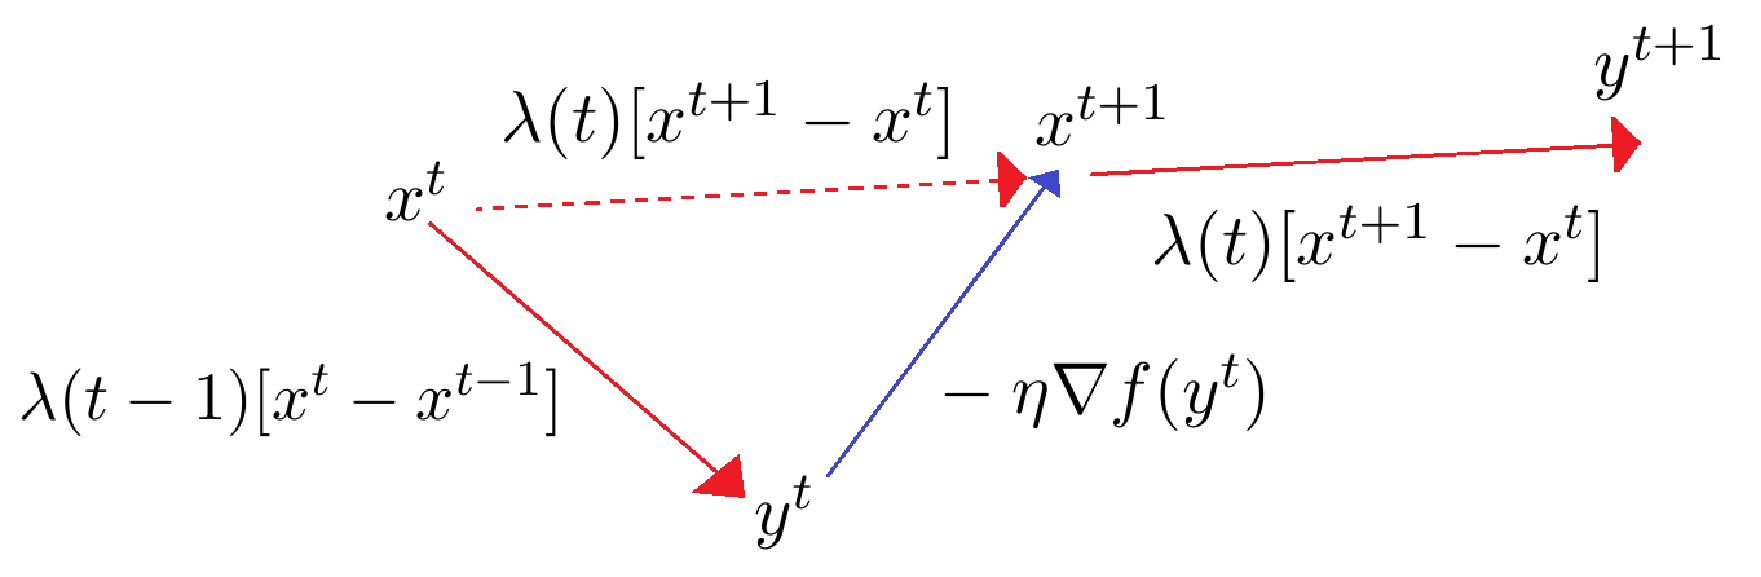
\includegraphics[width=0.6\textwidth]{./figures/iteracion}
\end{center}

Además que como se verá más adelante (en los resultados se observará claramente) el método de Nesterov lo que hace es ir oscilando en los alrededores del optimo, a diferencia del método del gradiente que se acerca solo por un lado por así decirlo. Presentaremos la siguiente figura para ilustrar: 

\begin{center}
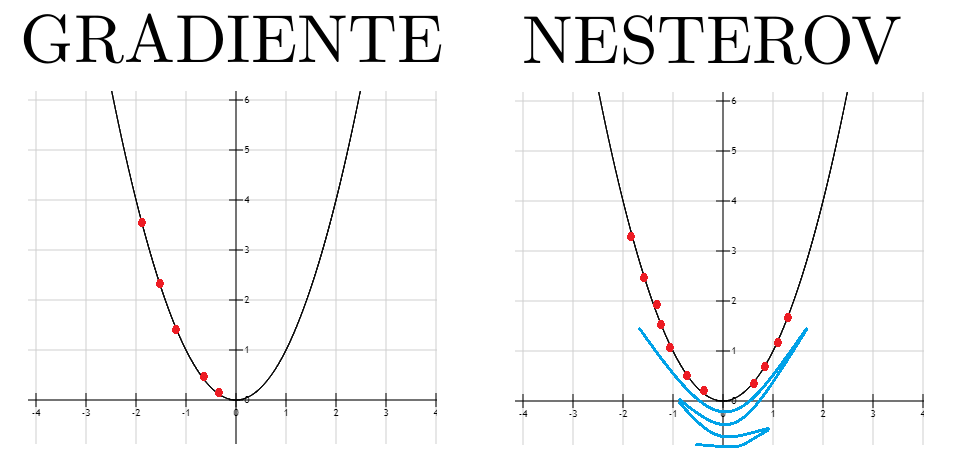
\includegraphics[width=0.6\textwidth]{./figures/gradne}
\end{center}

Como se observa el método del Gradiente solo se acerca por la izquierda y el método de Nesterov se acerca por ambos lados. La linea azul del gráfico de Nesterov es para indicar como se mueven los puntos en cada iteración, es decir, desde la izquierda a la derecha constantemente. El gráfico claramente es para un plano en $2D$ y se hizo para ejemplificar la idea de una manera visible. \\ 

Ahora comenzaremos el reporte de resultados. Es importante notar que usaremos de aquí en adelante la norma 2 ($  \left\| \right\|_2 $).

\hrulefill

\newpage

\subsection*{Reporte de resultados}

Lo primero que diremos es que para todos los graficos que realizaremos, el Método del Gradiente estara representado por el gráfico rojo, el Método de Backtracking por el color azul y el Método de Nesterov con el color verde. Lo que se está graficando son los errores que se indican para cada gráfico. \\

\textbf{i. Matriz A10 y vector b10:} \\

Es importante notar que tanto el método del gradiente como el Método de Nesterov calculaban el valor de $\mu$, que para esta función en particular corresponde al mayor valor propio asociado a la matriz respectiva. Para este caso la constante de suavidad $(\mu)$ corresponde a:

\[ \mu = 10.441263019930012 \] \

La cantidad de iteraciones que se realizaron fueron $T=1000$. \\

a) Lo primero que haremos será graficar $ f(x^T) - f^{*}$ para toda iteración $T$. El gráfico es:

\begin{center}
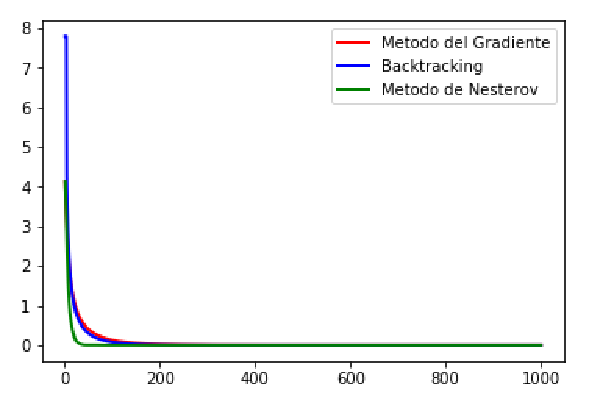
\includegraphics[width=0.6\textwidth]{./figures/grafico1}
\end{center}

\underline{Observación:} Como se observa, en el gráfico no se pueden distinguir mucho las diferentes curvas dado a que la magnitud de los errores es muy similar, por ende, pasaremos a graficar en escala logaritmica para poder diferenciar los distintos errores. \\

\newpage

b) Ahora graficaremos el logaritmo de $ f(x^T) - f^{*}$ para toda iteración $T$. El gráfico es:

\begin{center}
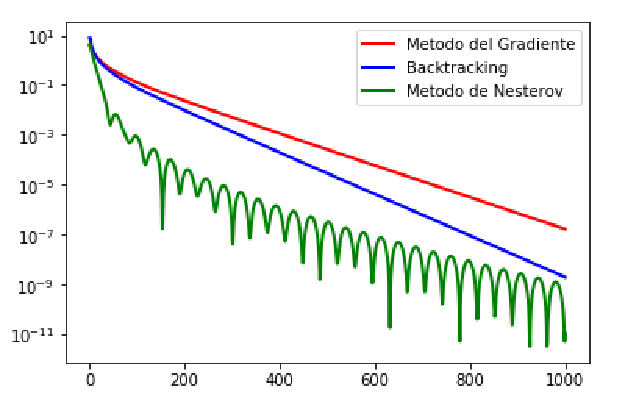
\includegraphics[width=0.6\textwidth]{./figures/grafico2}
\end{center}

\underline{Observación:} Es claro que tanto el método de backtracking como el método del gradiente tienen errores que decrecen de manera exponencial. Se observa que el método de backtracking siempre posee errores menores que el método del gradiente. Por otro lado, se observa que el método de Nesterov tiene oscilaciones en el valor de sus errores, sin embargo, estos errores son siempre menores que los errores del método de backtracking y del método del gradiente.   \\


c) Graficaremos también cual es la diferencia en norma 2 entre el $x^{*}$ y $x^T$ para todo $T$ \\

\begin{center}
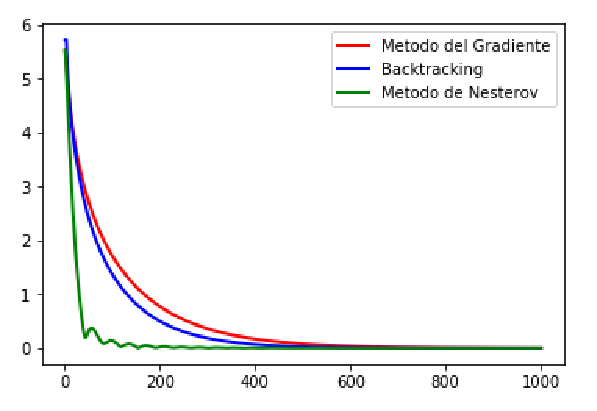
\includegraphics[width=0.6\textwidth]{./figures/grafico3}
\end{center}

\underline{Observación:} Notemos que el método de Nesterov posee un error que es mucho menor que el del método de backtracking y que el método del gradiente. Nuevamente el método de bakctracking posee un error que es menor que el del método del gradiente. Pasaremos a ver estos errores en escala logarítmica para observar de mejor manera sus comportamientos. \\

\newpage

d) Ahora graficaremos en escala logaritmica cual es la diferencia en norma 2 entre el $x^{*}$ y $x^T$ para todo $T$ \\

\begin{center}
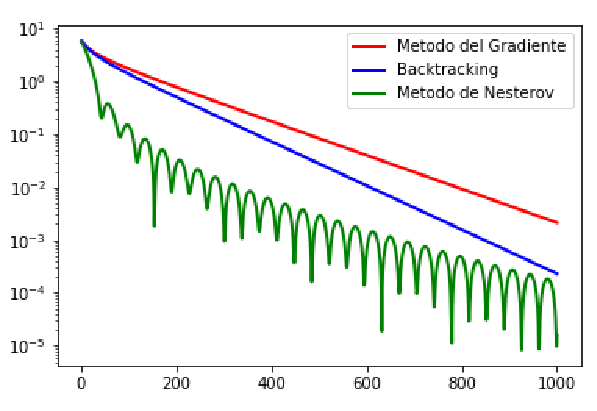
\includegraphics[width=0.6\textwidth]{./figures/grafico4}
\end{center}

\underline{Observación:} Al igual que en el gráfico $b)$ tanto el método de backtracking como el método del gradiente tienen errores que decrecen de manera exponencial. Se observa que el método de backtracking siempre posee errores menores que el método del gradiente. También, se observa que el método de Nesterov tiene oscilaciones en el valor de sus errores, sin embargo, estos errores son siempre menores que los errores del método de backtracking y del método del gradiente. \\

\textbf{ii. Matriz A100 y vector b100:} \\

Es importante notar que tanto el método del gradiente como el Método de Nesterov calculaban el valor de $\mu$, que para esta función en particular corresponde al mayor valor propio asociado a la matriz respectiva. Para este caso la constante de suavidad $(\mu)$ corresponde a:

\[ \mu = 100.5027345916198 \] \

La cantidad de iteraciones que se realizaron fueron $T=1000$. \\

\newpage

a) Lo primero que haremos será graficar $ f(x^T) - f^{*}$ para toda iteración $T$. El gráfico es:

\begin{center}
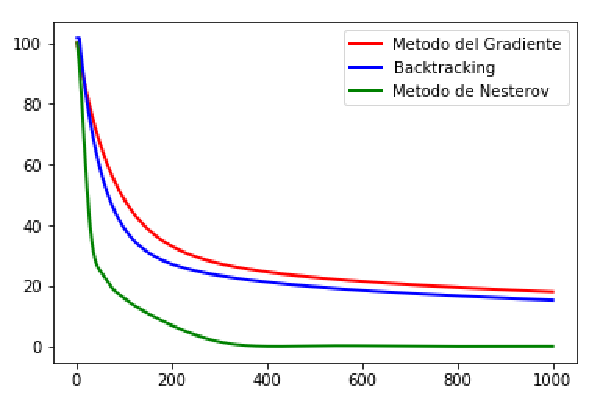
\includegraphics[width=0.6\textwidth]{./figures/grafico5}
\end{center}

\underline{Observación:} Se observa que el método de backtracking y el método del gradiente poseen errores que decrecen de manera similar, aunque nuevamente el método de backtracking posee errores menores que el método del gradiente. Mientras tanto, el método de Nesterov posee un decrecimiento que es mucho menor que el de los otros dos métodos.  \\

b) Ahora graficaremos el logaritmo de $ f(x^T) - f^{*}$ para toda iteración $T$. El gráfico es:

\begin{center}
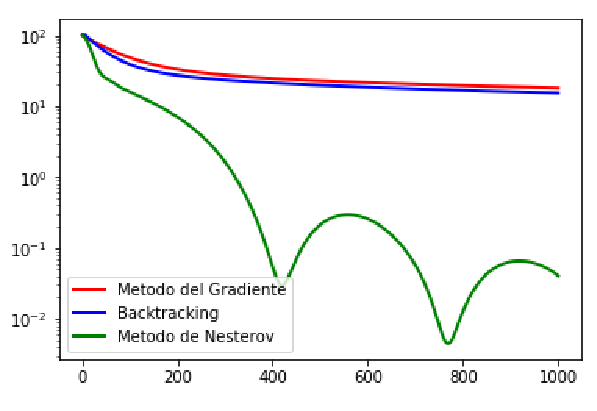
\includegraphics[width=0.6\textwidth]{./figures/grafico6}
\end{center}

\underline{Observación:} Como ya se había nombrado anteriormente, el método del gradiente y backtracking poseen errores muy similares y en escala logarítmica esto es más evidente aún. El método de Nesterov como ya se había nombrado antes posee errores menores que los otros dos métodos y nuevamente estos errores oscilan. \\

\newpage

c) Graficaremos también cual es la diferencia en norma 2 entre el $x^{*}$ y $x^T$ para todo $T$ \\

\begin{center}
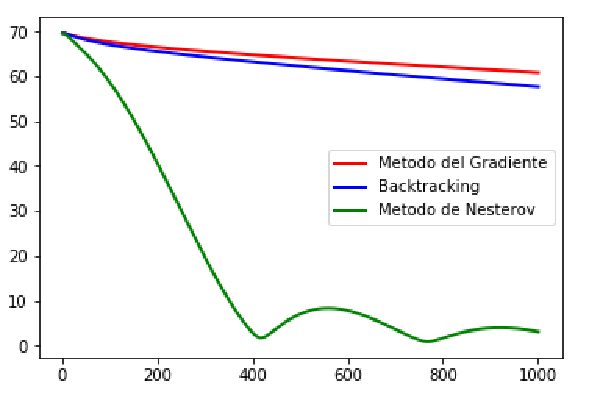
\includegraphics[width=0.6\textwidth]{./figures/grafico7}
\end{center}

\underline{Observación:} Se observa que tanto el método del gradiente como el método de backtracking poseen errores muy similares, mientras que el método de Nesterov posee errores que son mucho menores que el de los otros dos métodos, y que además oscilan.  \\

d) Ahora graficaremos en escala logaritmica cual es la diferencia en norma 2 entre el $x^{*}$ y $x^T$ para todo $T$ \\

\begin{center}
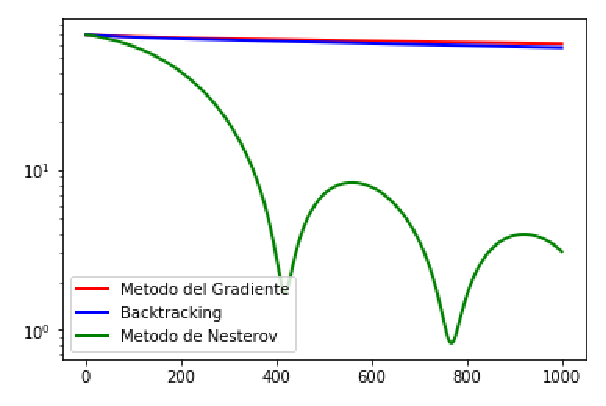
\includegraphics[width=0.6\textwidth]{./figures/grafico8}
\end{center}

\underline{Observación:} En escala logaritmica se hace más evidente la semejanza entre los errores de backtracking y del método del gradiente. Al igual que en el gráfico anterior, se observa que los errores de Nesterov oscilan y son menores que los de los otros dos métodos. \\

\newpage

\textbf{iii. Matriiz A1000 y vector b1000:} \\

Es importante notar que tanto el método del gradiente como el Método de Nesterov calculaban el valor de $\mu$, que para esta función en particular corresponde al mayor valor propio asociado a la matriz respectiva. Para este caso la constante de suavidad $(\mu)$ corresponde a:

\[ \mu = 1000.5144032964193 \] \

La cantidad de iteraciones que se realizaron fueron $T=100$. \\

a) Lo primero que haremos será graficar $ f(x^T) - f^{*}$ para toda iteración $T$. El gráfico es:

\begin{center}
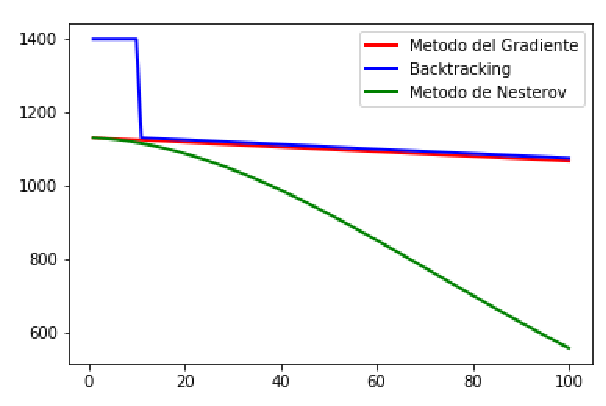
\includegraphics[width=0.6\textwidth]{./figures/grafico9}
\end{center}

\underline{Observación:} Se observa que el método de backtracking se mantiene constante hasta que encuentra un $\eta$ valido y luego de eso se observa que tanto los errores del método del gradiente como los de backtracking son similares y se ven medianamente constantes durante el tiempo, lo que indica que no esta habiendo convergencia. Por otro lado, el método de Nesterov posee errores menores que los otros dos métodos y estos errores van decreciendo lo que indica convergencia.  \\

\newpage

b) Ahora graficaremos el logaritmo de $ f(x^T) - f^{*}$ para toda iteración $T$. El gráfico es:

\begin{center}
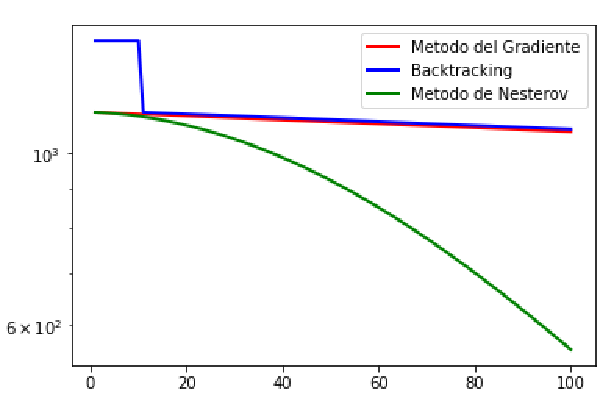
\includegraphics[width=0.6\textwidth]{./figures/grafico10}
\end{center}

\underline{Observación:} Al igual que en el gráfico anterior lo primero que se observa es que el método de backtracking se mantiene constante hasta que encuentra un $\eta$ valido y luego de eso sus errores se comportan muy similar a los del método del gradiente y estos son medianamente constantes lo que indica que no hay convergencia. Por otro lado, el método de Nesterov posee errores menores que los otros dos métodos los cuales van decreciendo, lo que indica convergencia. \\

c) Graficaremos también cual es la diferencia en norma 2 entre el $x^{*}$ y $x^T$ para todo $T$ \\

\begin{center}
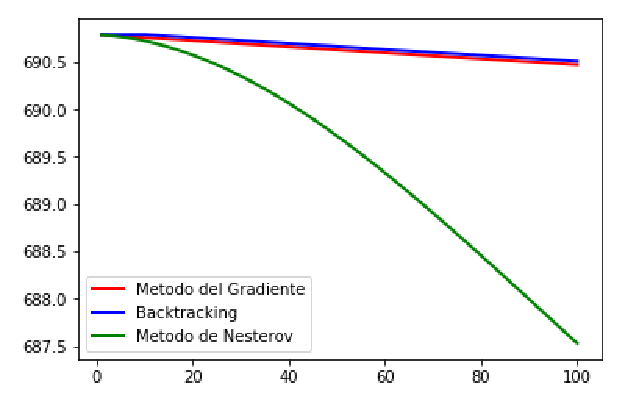
\includegraphics[width=0.6\textwidth]{./figures/grafico11}
\end{center}

\underline{Observación:} Al igual que en el caso anterior, los errores del método del gradiente y los de backtracking son muy similares y como estos se mantienen constante, se puede deducir que no hay convergencia, a diferencia del metodo de Nesterov que se ve que tiene errores que siempre decrecen lo cual indica convergencia. \\

\newpage

d) Ahora graficaremos en escala logaritmica cual es la diferencia en norma 2 entre el $x^{*}$ y $x^T$ para todo $T$ \\

\begin{center}
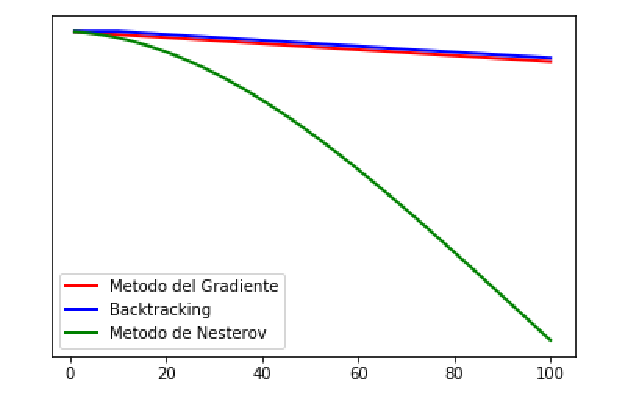
\includegraphics[width=0.6\textwidth]{./figures/grafico12}
\end{center}

\underline{Observación:} Al igual que en el caso anterior los errores del método del gradiente y de backtracking son muy similares y medianamente constantes lo que indica que no hay convergencia. Por otro lado, se observa que el método de Nesterov posee errores que decrecen continuamente lo cual nos permite deducir convergencia. \\

\begin{center}
\textbf{Conclusiones Generales}
\end{center}

En general lo que pudimos observar en todos los casos que analizamos es que la norma de la diferencia entre el $x^T$ generado por un método especifico y $x*$ (x optimo) se comportan muy similar a como se comporta la diferencia entre $f(x^T)$ y $ f(x^*) = f^*$. \\

En absolutamente todos los casos que se analizaron el método de Nesterov fue el que presento menores errores obteniendo muy buenos resultados a excepción del caso de $A1000$ y $b1000$ donde a pesar de que los errores iban decreciendo, estos estaban en valores cercanos a $600$ tanto para el error en $x$ ($\left\| x^T-x^{*} \right\|_2^2$) como para el error en $f$ ($f(x^T)-f^{*}$). Es importante de todos modos considerar que para $A1000$ y $b1000$ se realizaron $100$ iteraciones a diferencia de los casos de $A100,b100$ y $A10,b10$ en los cuales se realizaron $1000$ iteraciones. Esto se dio básicamente porque el computador en el que se estaban ejecutando los programas se demoraba mucho si considerabamos $T=1000$ en $A1000,b1000$. El método de Nesterov tiene la particularidad de que los errores van subiendo y bajando, es decir, oscilan, a diferencia de los otros métodos que hemos visto, los cuales siempre van disminuyendo sus errores de manera monótona, aunque estos mismos métodos son menos eficientes. Esto de alguna manera nos abre la posibilidad de contar y utilizar métodos más sofisticados que tienen errores que no decrecen de manera monótona, los cuales podrían llegar a ser más eficientes que los métodos con errores que decrecen de manera monótona.   \\

\newpage

Por otro lado, se observa que el método del backtracking y el método del gradiente se comportan muy similares, tanto cuando convergen como cuando no. De hecho, en estos ejemplos se observaron casos donde ambos métodos convergían y el método de backtracking lo hacía de mejor manera (poseía errores menores), a pesar de que en el método del gradiente poseíamos más información (el valor de la constante de suavidad). \\

Tanto el método del gradiente como el método de backtracing presentaron problemas en el sentido de que su error se mantenía constante para la matriz $A1000$, de lo cual podiamos deducir que no había convergencia, a diferencia del método de Nesterov que con ninguna matriz presento errores en cuanto a convergencia. De esta forma, podemos deducir que el método de Nesterov es capaz de operar con matrices más grandes que los otros dos métodos.  \\

\end{document}
